\chapter{Model Development}\label{ch:model_development}
In this chapter two models are developed based on the simple LSTM model from the silicon-valley-data-science RNN tutorial \cite{rubashkin2017}. Firstly these models (including their simple LSTM model) will be trained and tested on a small data set with the numbers:\\\\
$\left\{zero, one, two, three, four, five, six, seven, eight, nine \right\}$,\\\\
the same data used in Chapter \ref{ch:machine_learning} for the parameter comparison. After that, the best performing model shall be picked for a more detailed discription (with code) and futher trainig with a bigger data set of the english language. 

\section{Neural Network Comparison}

\begin{table}[H]
\centering
	\caption{Models.}
	\begin{tabular}{ l  c }
	Model1 -\tikzcircle[pink, fill=pink]{3pt}- &
	(Their simpleLSTM Model)\\
	Model2 -\tikzcircle[red, fill=red]{3pt}- &
	(Our simpleLSTM Model)\\
	Model3 -\tikzcircle[turquoise, fill=turquoise]{3pt}- &
	(Our BiRNN Model)\\
	\end{tabular}
	\label{tab:3_models}
\end{table}


\begin{table}[H]
\centering
    \caption{Parameter values of the three model.}
    \begin{tabular}{| l | c | c | c | c |} 
    \hline
        Parameters & 
        Model1 -\tikzcircle[pink, fill=pink]{3pt}- &
        Model2 -\tikzcircle[red, fill=red]{3pt}- &
        Model3 -\tikzcircle[turquoise, fill=turquoise]{3pt}-\\
    \hline
        Batch Size & 
        50 \hfill 20 \hfill 20 & 
        50 \hfill 20 \hfill 20 & 
        50 \hfill 20 \hfill 20 \\
    \hline
        Dropout & 
        0.05 & 0.05 & 0.05 \\
    \hline
        Learning Rate & 
        0.001 & 0.001 & 0.001 \\ 
    \hline
    \end{tabular}
    \label{tab:3models_tab}
\end{table}

\begin{figure}[H]
	\centering
	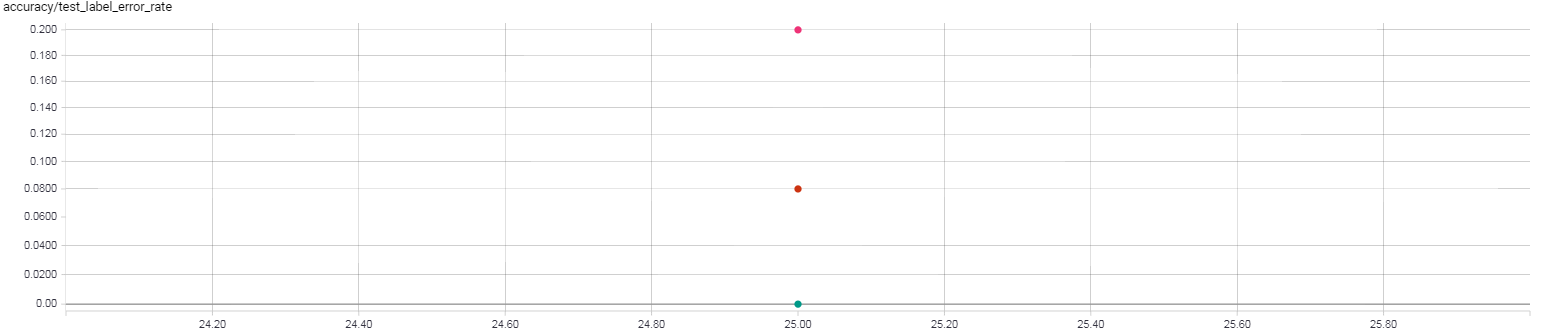
\includegraphics[width=\textwidth]		
	{model_development/3models_comparison/test_error_rate_3models}
	\caption{Test error rate.}
\end{figure}

\begin{figure}[H]
	\centering
	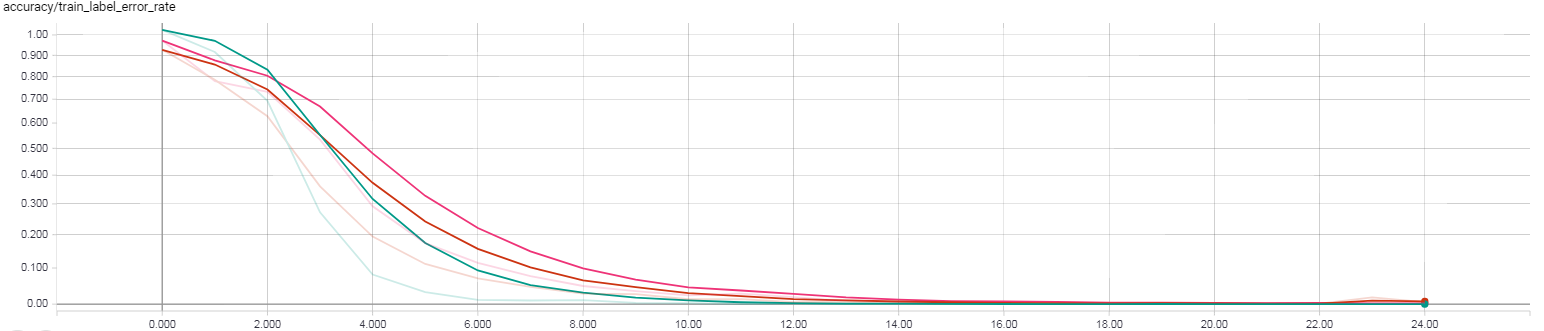
\includegraphics[width=\textwidth]		
	{model_development/3models_comparison/train_error_rate_3models}
	\caption{Training error rate.}
\end{figure}

\begin{figure}[H]
	\centering
	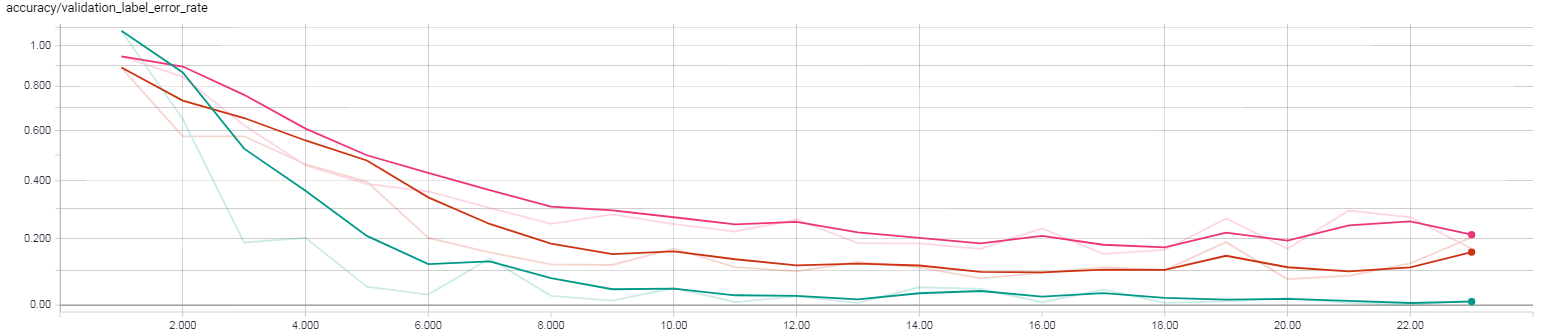
\includegraphics[width=\textwidth]		
	{model_development/3models_comparison/validation_error_rate_3models}
	\caption{Validation error rate.}
\end{figure}

\begin{figure}[H]
	\centering
	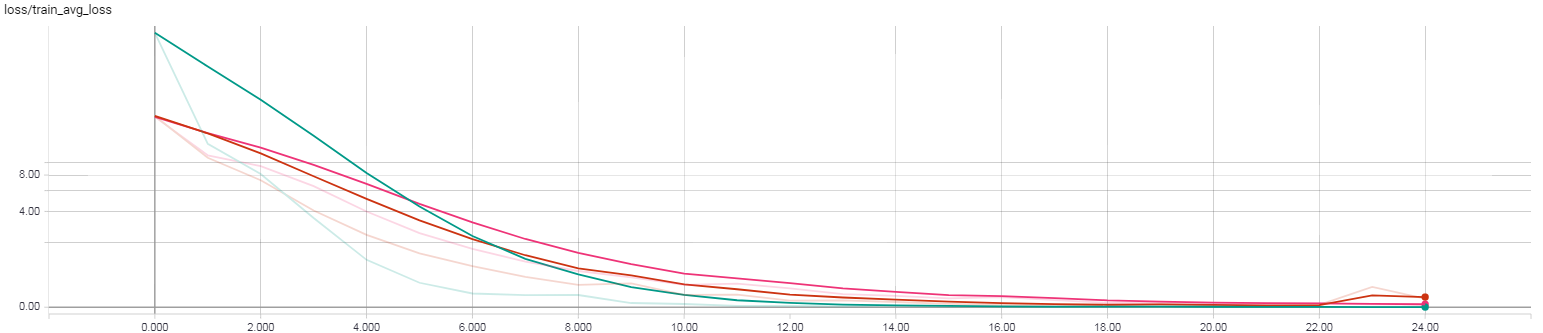
\includegraphics[width=\textwidth]		
	{model_development/3models_comparison/train_avg_loss_3models}
	\caption{Training average loss.}
\end{figure}

\section{Model Description}

One of the goals for this project was to research, design and compare different neural network topologies. 
Some of these were feed-forward, convolutional and recurrent. 
Continuing, some neural networks were made deep, first by adding fully connected layers to the existing type (feed-forward, CNN or RNN), and later, by changing the type (LSTM, GRU or BiRNN) and/or adding more main layers. 
Many such configurations were tested, some proving to be efficient for achieving designated goals, and some less so. \\\\
As shown in a previous chapter, \todo{reference which chapter we talk about} the model that is used in this DSR system is a recurrent neural network. 
This recurrent network is based on the standard LSTM cell, but used as a bidirectional layer. 
The purpose is to recognize the context of the text, to improve the prediction. 
The complete topology for the network is as follows: \\\\
\todo{INSERT NICE PICTURE DESCRIPTION HERE} \\\\
Described in figure X is the complete topology of the network used in the current implementation. It has a structure of 2-BiRNN-1-logits. In the beginning it has 2 fully connected layers, each consisting of 1024 neurons.
\lstinputlisting[language=Python, firstline=36, lastline=51]{code/txtFileMaker.py} 
Further on, the input is reshaped to be compatible with the BiRNN layer, consisting of two LSTM cells, each with 1024 neurons.
One cell is used in the "forward" direction, and the other one in the "backward" direction, with the goal of understanding the current context.
Following this step, the input is reshaped again and sent to the next fully connected layer.
The final layer, the logits layer, is used as output of the network. At this point, the original input is transformed by every layer and sent for decoding.
\todo{add caption}
\todo{clarify types of nn}

Model3 (BiRNN) is better therefore we go into more detail about it...
\todo{Make full page png}
\begin{figure}[H]
	\centering
	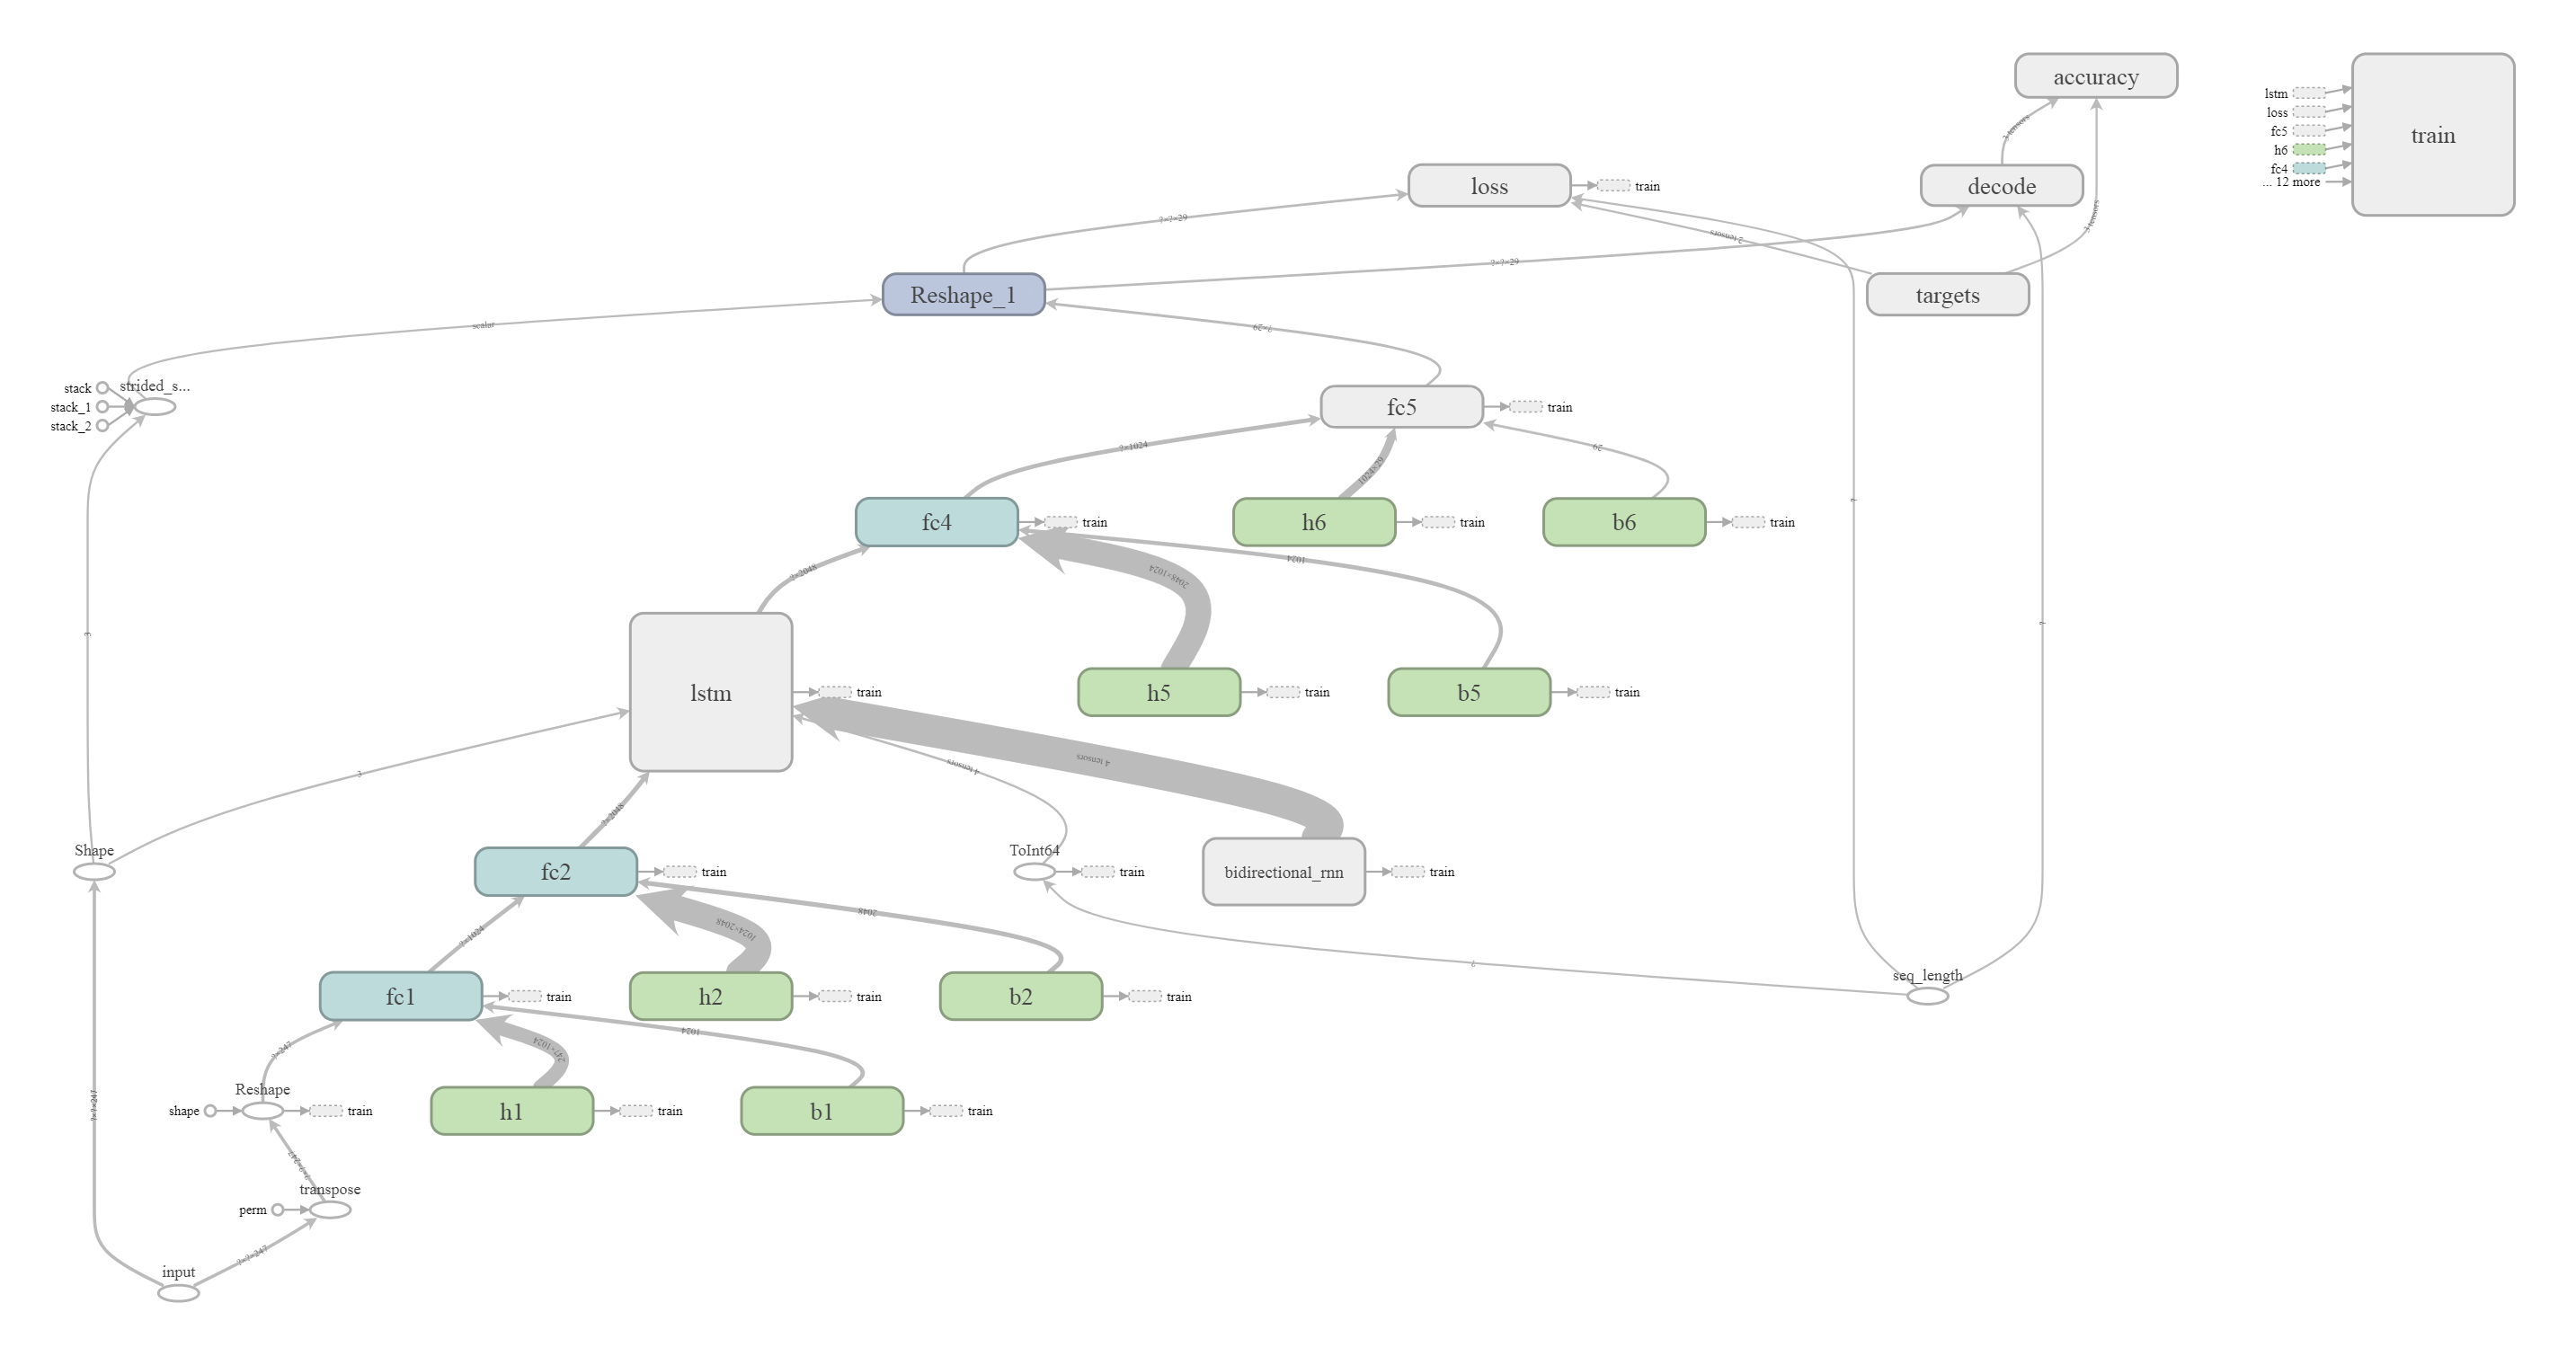
\includegraphics[width=\textwidth]		
	{model_development/birnn_v2_graph}
	\caption{Training average loss.}
\end{figure}